\documentclass[1p]{elsarticle_modified}
%\bibliographystyle{elsarticle-num}

%\usepackage[colorlinks]{hyperref}
%\usepackage{abbrmath_seonhwa} %\Abb, \Ascr, \Acal ,\Abf, \Afrak
\usepackage{amsfonts}
\usepackage{amssymb}
\usepackage{amsmath}
\usepackage{amsthm}
\usepackage{scalefnt}
\usepackage{amsbsy}
\usepackage{kotex}
\usepackage{caption}
\usepackage{subfig}
\usepackage{color}
\usepackage{graphicx}
\usepackage{xcolor} %% white, black, red, green, blue, cyan, magenta, yellow
\usepackage{float}
\usepackage{setspace}
\usepackage{hyperref}

\usepackage{tikz}
\usetikzlibrary{arrows}

\usepackage{multirow}
\usepackage{array} % fixed length table
\usepackage{hhline}

%%%%%%%%%%%%%%%%%%%%%
\makeatletter
\renewcommand*\env@matrix[1][\arraystretch]{%
	\edef\arraystretch{#1}%
	\hskip -\arraycolsep
	\let\@ifnextchar\new@ifnextchar
	\array{*\c@MaxMatrixCols c}}
\makeatother %https://tex.stackexchange.com/questions/14071/how-can-i-increase-the-line-spacing-in-a-matrix
%%%%%%%%%%%%%%%

\usepackage[normalem]{ulem}

\newcommand{\msout}[1]{\ifmmode\text{\sout{\ensuremath{#1}}}\else\sout{#1}\fi}
%SOURCE: \msout is \stkout macro in https://tex.stackexchange.com/questions/20609/strikeout-in-math-mode

\newcommand{\cancel}[1]{
	\ifmmode
	{\color{red}\msout{#1}}
	\else
	{\color{red}\sout{#1}}
	\fi
}

\newcommand{\add}[1]{
	{\color{blue}\uwave{#1}}
}

\newcommand{\replace}[2]{
	\ifmmode
	{\color{red}\msout{#1}}{\color{blue}\uwave{#2}}
	\else
	{\color{red}\sout{#1}}{\color{blue}\uwave{#2}}
	\fi
}

\newcommand{\Sol}{\mathcal{S}} %segment
\newcommand{\D}{D} %diagram
\newcommand{\A}{\mathcal{A}} %arc


%%%%%%%%%%%%%%%%%%%%%%%%%%%%%5 test

\def\sl{\operatorname{\textup{SL}}(2,\Cbb)}
\def\psl{\operatorname{\textup{PSL}}(2,\Cbb)}
\def\quan{\mkern 1mu \triangleright \mkern 1mu}

\theoremstyle{definition}
\newtheorem{thm}{Theorem}[section]
\newtheorem{prop}[thm]{Proposition}
\newtheorem{lem}[thm]{Lemma}
\newtheorem{ques}[thm]{Question}
\newtheorem{cor}[thm]{Corollary}
\newtheorem{defn}[thm]{Definition}
\newtheorem{exam}[thm]{Example}
\newtheorem{rmk}[thm]{Remark}
\newtheorem{alg}[thm]{Algorithm}

\newcommand{\I}{\sqrt{-1}}
\begin{document}

%\begin{frontmatter}
%
%\title{Boundary parabolic representations of knots up to 8 crossings}
%
%%% Group authors per affiliation:
%\author{Yunhi Cho} 
%\address{Department of Mathematics, University of Seoul, Seoul, Korea}
%\ead{yhcho@uos.ac.kr}
%
%
%\author{Seonhwa Kim} %\fnref{s_kim}}
%\address{Center for Geometry and Physics, Institute for Basic Science, Pohang, 37673, Korea}
%\ead{ryeona17@ibs.re.kr}
%
%\author{Hyuk Kim}
%\address{Department of Mathematical Sciences, Seoul National University, Seoul 08826, Korea}
%\ead{hyukkim@snu.ac.kr}
%
%\author{Seokbeom Yoon}
%\address{Department of Mathematical Sciences, Seoul National University, Seoul, 08826,  Korea}
%\ead{sbyoon15@snu.ac.kr}
%
%\begin{abstract}
%We find all boundary parabolic representation of knots up to 8 crossings.
%
%\end{abstract}
%\begin{keyword}
%    \MSC[2010] 57M25 
%\end{keyword}
%
%\end{frontmatter}

%\linenumbers
%\tableofcontents
%
\newcommand\colored[1]{\textcolor{white}{\rule[-0.35ex]{0.8em}{1.4ex}}\kern-0.8em\color{red} #1}%
%\newcommand\colored[1]{\textcolor{white}{ #1}\kern-2.17ex	\textcolor{white}{ #1}\kern-1.81ex	\textcolor{white}{ #1}\kern-2.15ex\color{red}#1	}

{\Large $\underline{11n_{46}~(K11n_{46})}$}

\setlength{\tabcolsep}{10pt}
\renewcommand{\arraystretch}{1.6}
\vspace{1cm}\begin{tabular}{m{100pt}>{\centering\arraybackslash}m{274pt}}
\multirow{5}{120pt}{
	\centering
	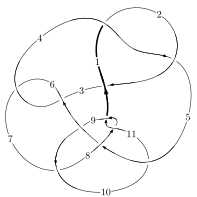
\includegraphics[width=112pt]{../../../GIT/diagram.site/Diagrams/png/662_11n_46.png}\\
\ \ \ A knot diagram\footnotemark}&
\allowdisplaybreaks
\textbf{Linearized knot diagam} \\
\cline{2-2}
 &
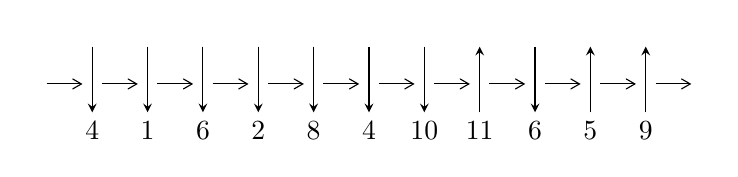
\begin{tikzpicture}[x=20pt, y=17pt]
	% nodes
	\node (C0) at (0, 0) {};
	\node (C1) at (1, 0) {};
	\node (C1U) at (1, +1) {};
	\node (C1D) at (1, -1) {4};

	\node (C2) at (2, 0) {};
	\node (C2U) at (2, +1) {};
	\node (C2D) at (2, -1) {1};

	\node (C3) at (3, 0) {};
	\node (C3U) at (3, +1) {};
	\node (C3D) at (3, -1) {6};

	\node (C4) at (4, 0) {};
	\node (C4U) at (4, +1) {};
	\node (C4D) at (4, -1) {2};

	\node (C5) at (5, 0) {};
	\node (C5U) at (5, +1) {};
	\node (C5D) at (5, -1) {8};

	\node (C6) at (6, 0) {};
	\node (C6U) at (6, +1) {};
	\node (C6D) at (6, -1) {4};

	\node (C7) at (7, 0) {};
	\node (C7U) at (7, +1) {};
	\node (C7D) at (7, -1) {10};

	\node (C8) at (8, 0) {};
	\node (C8U) at (8, +1) {};
	\node (C8D) at (8, -1) {11};

	\node (C9) at (9, 0) {};
	\node (C9U) at (9, +1) {};
	\node (C9D) at (9, -1) {6};

	\node (C10) at (10, 0) {};
	\node (C10U) at (10, +1) {};
	\node (C10D) at (10, -1) {5};

	\node (C11) at (11, 0) {};
	\node (C11U) at (11, +1) {};
	\node (C11D) at (11, -1) {9};
	\node (C12) at (12, 0) {};

	% arrows
	\draw[->,>={angle 60}]
	(C0) edge (C1) (C1) edge (C2) (C2) edge (C3) (C3) edge (C4) (C4) edge (C5) (C5) edge (C6) (C6) edge (C7) (C7) edge (C8) (C8) edge (C9) (C9) edge (C10) (C10) edge (C11) (C11) edge (C12) ;	\draw[->,>=stealth]
	(C1U) edge (C1D) (C2U) edge (C2D) (C3U) edge (C3D) (C4U) edge (C4D) (C5U) edge (C5D) (C6U) edge (C6D) (C7U) edge (C7D) (C8D) edge (C8U) (C9U) edge (C9D) (C10D) edge (C10U) (C11D) edge (C11U) ;
	\end{tikzpicture} \\
\hhline{~~} \\& 
\textbf{Solving Sequence} \\ \cline{2-2} 
 &
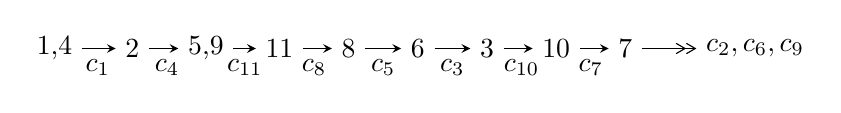
\begin{tikzpicture}[x=25pt, y=7pt]
	% node
	\node (A0) at (-1/8, 0) {1,4};
	\node (A1) at (1, 0) {2};
	\node (A2) at (33/16, 0) {5,9};
	\node (A3) at (25/8, 0) {11};
	\node (A4) at (33/8, 0) {8};
	\node (A5) at (41/8, 0) {6};
	\node (A6) at (49/8, 0) {3};
	\node (A7) at (57/8, 0) {10};
	\node (A8) at (65/8, 0) {7};
	\node (C1) at (1/2, -1) {$c_{1}$};
	\node (C2) at (3/2, -1) {$c_{4}$};
	\node (C3) at (21/8, -1) {$c_{11}$};
	\node (C4) at (29/8, -1) {$c_{8}$};
	\node (C5) at (37/8, -1) {$c_{5}$};
	\node (C6) at (45/8, -1) {$c_{3}$};
	\node (C7) at (53/8, -1) {$c_{10}$};
	\node (C8) at (61/8, -1) {$c_{7}$};
	\node (A9) at (10, 0) {$c_{2},c_{6},c_{9}$};

	% edge
	\draw[->,>=stealth]	
	(A0) edge (A1) (A1) edge (A2) (A2) edge (A3) (A3) edge (A4) (A4) edge (A5) (A5) edge (A6) (A6) edge (A7) (A7) edge (A8) ;
	\draw[->>,>={angle 60}]	
	(A8) edge (A9);
\end{tikzpicture} \\ 

\end{tabular} \\

\footnotetext{
The image of knot diagram is generated by the software ``\textbf{Draw programme}" developed by Andrew Bartholomew(\url{http://www.layer8.co.uk/maths/draw/index.htm\#Running-draw}), where we modified some parts for our purpose(\url{https://github.com/CATsTAILs/LinksPainter}).
}\phantom \\ \newline 
\centering \textbf{Ideals for irreducible components\footnotemark of $X_{\text{par}}$} 
 
\begin{align*}
I^u_{1}&=\langle 
-5.02472\times10^{36} u^{46}-3.62196\times10^{37} u^{45}+\cdots+8.54755\times10^{36} b-2.09417\times10^{36},\\
\phantom{I^u_{1}}&\phantom{= \langle  }-5.51836\times10^{36} u^{46}-4.22287\times10^{37} u^{45}+\cdots+8.54755\times10^{36} a+5.43355\times10^{37},\;u^{47}+8 u^{46}+\cdots+7 u+1\rangle \\
I^u_{2}&=\langle 
b- a+1,\;a^6-5 a^5+9 a^4-8 a^3+5 a^2-2 a+1,\;u-1\rangle \\
I^u_{3}&=\langle 
b-1,\;a+4 u+7,\;u^2+u-1\rangle \\
\\
\end{align*}
\raggedright * 3 irreducible components of $\dim_{\mathbb{C}}=0$, with total 55 representations.\\
\footnotetext{All coefficients of polynomials are rational numbers. But the coefficients are sometimes approximated in decimal forms when there is not enough margin.}
\newpage
\renewcommand{\arraystretch}{1}
\centering \section*{I. $I^u_{1}= \langle -5.02\times10^{36} u^{46}-3.62\times10^{37} u^{45}+\cdots+8.55\times10^{36} b-2.09\times10^{36},\;-5.52\times10^{36} u^{46}-4.22\times10^{37} u^{45}+\cdots+8.55\times10^{36} a+5.43\times10^{37},\;u^{47}+8 u^{46}+\cdots+7 u+1 \rangle$}
\flushleft \textbf{(i) Arc colorings}\\
\begin{tabular}{m{7pt} m{180pt} m{7pt} m{180pt} }
\flushright $a_{1}=$&$\begin{pmatrix}1\\0\end{pmatrix}$ \\
\flushright $a_{4}=$&$\begin{pmatrix}0\\u\end{pmatrix}$ \\
\flushright $a_{2}=$&$\begin{pmatrix}1\\u^2\end{pmatrix}$ \\
\flushright $a_{5}=$&$\begin{pmatrix}- u\\- u^3+u\end{pmatrix}$ \\
\flushright $a_{9}=$&$\begin{pmatrix}0.645608 u^{46}+4.94044 u^{45}+\cdots-39.0274 u-6.35686\\0.587855 u^{46}+4.23742 u^{45}+\cdots+6.17462 u+0.245002\end{pmatrix}$ \\
\flushright $a_{11}=$&$\begin{pmatrix}0.809363 u^{46}+5.77890 u^{45}+\cdots+51.2482 u+7.31402\\0.917596 u^{46}+6.82877 u^{45}+\cdots+8.41124 u+2.05442\end{pmatrix}$ \\
\flushright $a_{8}=$&$\begin{pmatrix}1.08058 u^{46}+8.14247 u^{45}+\cdots+9.68656 u-1.51066\\0.508743 u^{46}+3.94324 u^{45}+\cdots+9.53527 u+1.05799\end{pmatrix}$ \\
\flushright $a_{6}=$&$\begin{pmatrix}0.377639 u^{46}+2.54848 u^{45}+\cdots-12.1966 u-0.249306\\0.653298 u^{46}+5.04572 u^{45}+\cdots+6.43493 u+1.03094\end{pmatrix}$ \\
\flushright $a_{3}=$&$\begin{pmatrix}- u^2+1\\u^2\end{pmatrix}$ \\
\flushright $a_{10}=$&$\begin{pmatrix}0.444835 u^{46}+2.50822 u^{45}+\cdots+42.3670 u+5.69307\\2.59653 u^{46}+19.3282 u^{45}+\cdots+20.1382 u+4.02983\end{pmatrix}$ \\
\flushright $a_{7}=$&$\begin{pmatrix}0.377639 u^{46}+2.54848 u^{45}+\cdots-12.1966 u-0.249306\\1.15585 u^{46}+8.72441 u^{45}+\cdots+9.36570 u+1.50357\end{pmatrix}$\\ \flushright $a_{7}=$&$\begin{pmatrix}0.377639 u^{46}+2.54848 u^{45}+\cdots-12.1966 u-0.249306\\1.15585 u^{46}+8.72441 u^{45}+\cdots+9.36570 u+1.50357\end{pmatrix}$\\&\end{tabular}
\flushleft \textbf{(ii) Obstruction class $= -1$}\\~\\
\flushleft \textbf{(iii) Cusp Shapes $= -7.05583 u^{46}-61.7041 u^{45}+\cdots+99.8008 u+14.7497$}\\~\\
\newpage\renewcommand{\arraystretch}{1}
\flushleft \textbf{(iv) u-Polynomials at the component}\newline \\
\begin{tabular}{m{50pt}|m{274pt}}
Crossings & \hspace{64pt}u-Polynomials at each crossing \\
\hline $$\begin{aligned}c_{1},c_{4}\end{aligned}$$&$\begin{aligned}
&u^{47}-8 u^{46}+\cdots+7 u-1
\end{aligned}$\\
\hline $$\begin{aligned}c_{2}\end{aligned}$$&$\begin{aligned}
&u^{47}+18 u^{46}+\cdots-3 u+1
\end{aligned}$\\
\hline $$\begin{aligned}c_{3},c_{6}\end{aligned}$$&$\begin{aligned}
&u^{47}-2 u^{46}+\cdots-64 u-64
\end{aligned}$\\
\hline $$\begin{aligned}c_{5}\end{aligned}$$&$\begin{aligned}
&u^{47}-3 u^{46}+\cdots+2 u-1
\end{aligned}$\\
\hline $$\begin{aligned}c_{7}\end{aligned}$$&$\begin{aligned}
&u^{47}-8 u^{46}+\cdots+48 u+4
\end{aligned}$\\
\hline $$\begin{aligned}c_{8},c_{11}\end{aligned}$$&$\begin{aligned}
&u^{47}+4 u^{46}+\cdots-11 u-1
\end{aligned}$\\
\hline $$\begin{aligned}c_{9}\end{aligned}$$&$\begin{aligned}
&u^{47}- u^{46}+\cdots-3568 u-5873
\end{aligned}$\\
\hline $$\begin{aligned}c_{10}\end{aligned}$$&$\begin{aligned}
&u^{47}+3 u^{46}+\cdots+698 u+191
\end{aligned}$\\
\hline
\end{tabular}\\~\\
\newpage\renewcommand{\arraystretch}{1}
\flushleft \textbf{(v) Riley Polynomials at the component}\newline \\
\begin{tabular}{m{50pt}|m{274pt}}
Crossings & \hspace{64pt}Riley Polynomials at each crossing \\
\hline $$\begin{aligned}c_{1},c_{4}\end{aligned}$$&$\begin{aligned}
&y^{47}-18 y^{46}+\cdots-3 y-1
\end{aligned}$\\
\hline $$\begin{aligned}c_{2}\end{aligned}$$&$\begin{aligned}
&y^{47}+30 y^{46}+\cdots-1935 y-1
\end{aligned}$\\
\hline $$\begin{aligned}c_{3},c_{6}\end{aligned}$$&$\begin{aligned}
&y^{47}+36 y^{46}+\cdots-61440 y-4096
\end{aligned}$\\
\hline $$\begin{aligned}c_{5}\end{aligned}$$&$\begin{aligned}
&y^{47}+y^{46}+\cdots+8 y-1
\end{aligned}$\\
\hline $$\begin{aligned}c_{7}\end{aligned}$$&$\begin{aligned}
&y^{47}+12 y^{46}+\cdots+1080 y-16
\end{aligned}$\\
\hline $$\begin{aligned}c_{8},c_{11}\end{aligned}$$&$\begin{aligned}
&y^{47}-38 y^{46}+\cdots+407 y-1
\end{aligned}$\\
\hline $$\begin{aligned}c_{9}\end{aligned}$$&$\begin{aligned}
&y^{47}-19 y^{46}+\cdots+74984424 y-34492129
\end{aligned}$\\
\hline $$\begin{aligned}c_{10}\end{aligned}$$&$\begin{aligned}
&y^{47}-59 y^{46}+\cdots+1536176 y-36481
\end{aligned}$\\
\hline
\end{tabular}\\~\\
\newpage\flushleft \textbf{(vi) Complex Volumes and Cusp Shapes}
$$\begin{array}{c|c|c}  
\text{Solutions to }I^u_{1}& \I (\text{vol} + \sqrt{-1}CS) & \text{Cusp shape}\\
 \hline 
\begin{aligned}
u &= \phantom{-}1.033480 + 0.093725 I \\
a &= -3.27954 + 1.31288 I \\
b &= -1.081150 + 0.125029 I\end{aligned}
 & \phantom{-}0.321927 - 0.588102 I & -6.8283 - 18.9142 I \\ \hline\begin{aligned}
u &= \phantom{-}1.033480 - 0.093725 I \\
a &= -3.27954 - 1.31288 I \\
b &= -1.081150 - 0.125029 I\end{aligned}
 & \phantom{-}0.321927 + 0.588102 I & -6.8283 + 18.9142 I \\ \hline\begin{aligned}
u &= -0.757104 + 0.786690 I \\
a &= -0.425941 + 0.514521 I \\
b &= -0.456029 + 0.425744 I\end{aligned}
 & \phantom{-}3.72033 + 1.52573 I & -5.00000 - 4.80548 I \\ \hline\begin{aligned}
u &= -0.757104 - 0.786690 I \\
a &= -0.425941 - 0.514521 I \\
b &= -0.456029 - 0.425744 I\end{aligned}
 & \phantom{-}3.72033 - 1.52573 I & -5.00000 + 4.80548 I \\ \hline\begin{aligned}
u &= \phantom{-}0.764975 + 0.478588 I \\
a &= \phantom{-}0.406292 - 0.390089 I \\
b &= -0.198952 + 0.856716 I\end{aligned}
 & -1.05831 - 3.36011 I & -6.88945 + 7.26716 I \\ \hline\begin{aligned}
u &= \phantom{-}0.764975 - 0.478588 I \\
a &= \phantom{-}0.406292 + 0.390089 I \\
b &= -0.198952 - 0.856716 I\end{aligned}
 & -1.05831 + 3.36011 I & -6.88945 - 7.26716 I \\ \hline\begin{aligned}
u &= -0.698652 + 0.895191 I \\
a &= -0.430113 - 0.271427 I \\
b &= -0.379185 + 1.269650 I\end{aligned}
 & \phantom{-}4.30107 - 2.55894 I & \phantom{-0.000000 } 0 \\ \hline\begin{aligned}
u &= -0.698652 - 0.895191 I \\
a &= -0.430113 + 0.271427 I \\
b &= -0.379185 - 1.269650 I\end{aligned}
 & \phantom{-}4.30107 + 2.55894 I & \phantom{-0.000000 } 0 \\ \hline\begin{aligned}
u &= \phantom{-}1.202260 + 0.035924 I \\
a &= -1.167100 - 0.796046 I \\
b &= -0.058543 - 0.584512 I\end{aligned}
 & -2.41059 + 1.46028 I & \phantom{-0.000000 } 0 \\ \hline\begin{aligned}
u &= \phantom{-}1.202260 - 0.035924 I \\
a &= -1.167100 + 0.796046 I \\
b &= -0.058543 + 0.584512 I\end{aligned}
 & -2.41059 - 1.46028 I & \phantom{-0.000000 } 0\\
 \hline 
 \end{array}$$\newpage$$\begin{array}{c|c|c}  
\text{Solutions to }I^u_{1}& \I (\text{vol} + \sqrt{-1}CS) & \text{Cusp shape}\\
 \hline 
\begin{aligned}
u &= -0.898968 + 0.805280 I \\
a &= \phantom{-}2.53734 - 1.10815 I \\
b &= -1.178330 - 0.064139 I\end{aligned}
 & \phantom{-}5.31855 + 3.02042 I & \phantom{-0.000000 } 0 \\ \hline\begin{aligned}
u &= -0.898968 - 0.805280 I \\
a &= \phantom{-}2.53734 + 1.10815 I \\
b &= -1.178330 + 0.064139 I\end{aligned}
 & \phantom{-}5.31855 - 3.02042 I & \phantom{-0.000000 } 0 \\ \hline\begin{aligned}
u &= -0.778806 + 0.103648 I \\
a &= \phantom{-}0.189578 + 0.862116 I \\
b &= \phantom{-}1.032870 + 0.611950 I\end{aligned}
 & -1.17157 + 5.91398 I & \phantom{-}2.20637 - 8.69493 I \\ \hline\begin{aligned}
u &= -0.778806 - 0.103648 I \\
a &= \phantom{-}0.189578 - 0.862116 I \\
b &= \phantom{-}1.032870 - 0.611950 I\end{aligned}
 & -1.17157 - 5.91398 I & \phantom{-}2.20637 + 8.69493 I \\ \hline\begin{aligned}
u &= \phantom{-}0.855886 + 0.862796 I \\
a &= -1.72616 - 0.65853 I \\
b &= \phantom{-}1.38287 - 0.35151 I\end{aligned}
 & \phantom{-}3.93862 - 7.66972 I & \phantom{-0.000000 } 0 \\ \hline\begin{aligned}
u &= \phantom{-}0.855886 - 0.862796 I \\
a &= -1.72616 + 0.65853 I \\
b &= \phantom{-}1.38287 + 0.35151 I\end{aligned}
 & \phantom{-}3.93862 + 7.66972 I & \phantom{-0.000000 } 0 \\ \hline\begin{aligned}
u &= -0.998921 + 0.724997 I \\
a &= -0.024266 - 0.535985 I \\
b &= -0.154567 - 0.525352 I\end{aligned}
 & \phantom{-}2.96538 + 4.21460 I & \phantom{-0.000000 } 0 \\ \hline\begin{aligned}
u &= -0.998921 - 0.724997 I \\
a &= -0.024266 + 0.535985 I \\
b &= -0.154567 + 0.525352 I\end{aligned}
 & \phantom{-}2.96538 - 4.21460 I & \phantom{-0.000000 } 0 \\ \hline\begin{aligned}
u &= -0.861156 + 0.894994 I \\
a &= \phantom{-}0.955021 - 0.682279 I \\
b &= -1.71720 + 0.56072 I\end{aligned}
 & \phantom{-}8.18563 + 0.96335 I & \phantom{-0.000000 } 0 \\ \hline\begin{aligned}
u &= -0.861156 - 0.894994 I \\
a &= \phantom{-}0.955021 + 0.682279 I \\
b &= -1.71720 - 0.56072 I\end{aligned}
 & \phantom{-}8.18563 - 0.96335 I & \phantom{-0.000000 } 0\\
 \hline 
 \end{array}$$\newpage$$\begin{array}{c|c|c}  
\text{Solutions to }I^u_{1}& \I (\text{vol} + \sqrt{-1}CS) & \text{Cusp shape}\\
 \hline 
\begin{aligned}
u &= \phantom{-}0.690875 + 0.281167 I \\
a &= -1.112220 + 0.602692 I \\
b &= -0.131471 - 0.129043 I\end{aligned}
 & -0.875787 - 0.039510 I & -8.12380 - 0.07387 I \\ \hline\begin{aligned}
u &= \phantom{-}0.690875 - 0.281167 I \\
a &= -1.112220 - 0.602692 I \\
b &= -0.131471 + 0.129043 I\end{aligned}
 & -0.875787 + 0.039510 I & -8.12380 + 0.07387 I \\ \hline\begin{aligned}
u &= -0.565814 + 1.147400 I \\
a &= -1.365050 + 0.208322 I \\
b &= \phantom{-}1.51205 - 0.45021 I\end{aligned}
 & \phantom{-}10.31450 - 8.43955 I & \phantom{-0.000000 } 0 \\ \hline\begin{aligned}
u &= -0.565814 - 1.147400 I \\
a &= -1.365050 - 0.208322 I \\
b &= \phantom{-}1.51205 + 0.45021 I\end{aligned}
 & \phantom{-}10.31450 + 8.43955 I & \phantom{-0.000000 } 0 \\ \hline\begin{aligned}
u &= -0.969617 + 0.854773 I \\
a &= \phantom{-}1.38412 - 1.02994 I \\
b &= -1.59947 - 0.76351 I\end{aligned}
 & \phantom{-}7.84802 + 5.50326 I & \phantom{-0.000000 } 0 \\ \hline\begin{aligned}
u &= -0.969617 - 0.854773 I \\
a &= \phantom{-}1.38412 + 1.02994 I \\
b &= -1.59947 + 0.76351 I\end{aligned}
 & \phantom{-}7.84802 - 5.50326 I & \phantom{-0.000000 } 0 \\ \hline\begin{aligned}
u &= \phantom{-}0.687161\phantom{ +0.000000I} \\
a &= \phantom{-}14.6161\phantom{ +0.000000I} \\
b &= -1.01048\phantom{ +0.000000I}\end{aligned}
 & \phantom{-}0.618242\phantom{ +0.000000I} & -202.120\phantom{ +0.000000I} \\ \hline\begin{aligned}
u &= \phantom{-}0.989321 + 0.869498 I \\
a &= -1.23050 - 0.78743 I \\
b &= \phantom{-}1.314120 + 0.116801 I\end{aligned}
 & \phantom{-}3.55960 + 1.25869 I & \phantom{-0.000000 } 0 \\ \hline\begin{aligned}
u &= \phantom{-}0.989321 - 0.869498 I \\
a &= -1.23050 + 0.78743 I \\
b &= \phantom{-}1.314120 - 0.116801 I\end{aligned}
 & \phantom{-}3.55960 - 1.25869 I & \phantom{-0.000000 } 0 \\ \hline\begin{aligned}
u &= -0.526112 + 1.208050 I \\
a &= -1.351960 + 0.132410 I \\
b &= \phantom{-}1.41271 - 0.07084 I\end{aligned}
 & \phantom{-}9.82610 + 0.01608 I & \phantom{-0.000000 } 0\\
 \hline 
 \end{array}$$\newpage$$\begin{array}{c|c|c}  
\text{Solutions to }I^u_{1}& \I (\text{vol} + \sqrt{-1}CS) & \text{Cusp shape}\\
 \hline 
\begin{aligned}
u &= -0.526112 - 1.208050 I \\
a &= -1.351960 - 0.132410 I \\
b &= \phantom{-}1.41271 + 0.07084 I\end{aligned}
 & \phantom{-}9.82610 - 0.01608 I & \phantom{-0.000000 } 0 \\ \hline\begin{aligned}
u &= -1.065440 + 0.776679 I \\
a &= \phantom{-}0.770185 - 0.171718 I \\
b &= -0.125387 - 1.358280 I\end{aligned}
 & \phantom{-}3.17396 + 8.77694 I & \phantom{-0.000000 } 0 \\ \hline\begin{aligned}
u &= -1.065440 - 0.776679 I \\
a &= \phantom{-}0.770185 + 0.171718 I \\
b &= -0.125387 + 1.358280 I\end{aligned}
 & \phantom{-}3.17396 - 8.77694 I & \phantom{-0.000000 } 0 \\ \hline\begin{aligned}
u &= -0.626077 + 0.139965 I \\
a &= -0.423419 + 1.223810 I \\
b &= \phantom{-}0.546092 + 0.803481 I\end{aligned}
 & -2.68564 - 0.62982 I & -2.91172 - 0.97884 I \\ \hline\begin{aligned}
u &= -0.626077 - 0.139965 I \\
a &= -0.423419 - 1.223810 I \\
b &= \phantom{-}0.546092 - 0.803481 I\end{aligned}
 & -2.68564 + 0.62982 I & -2.91172 + 0.97884 I \\ \hline\begin{aligned}
u &= -1.21414 + 0.79886 I \\
a &= -1.25398 + 1.21055 I \\
b &= \phantom{-}1.47839 + 0.56828 I\end{aligned}
 & \phantom{-}8.2500 + 15.4047 I & \phantom{-0.000000 } 0 \\ \hline\begin{aligned}
u &= -1.21414 - 0.79886 I \\
a &= -1.25398 - 1.21055 I \\
b &= \phantom{-}1.47839 - 0.56828 I\end{aligned}
 & \phantom{-}8.2500 - 15.4047 I & \phantom{-0.000000 } 0 \\ \hline\begin{aligned}
u &= \phantom{-}0.434172 + 0.311062 I \\
a &= \phantom{-}2.92847 - 0.34363 I \\
b &= -1.301780 + 0.320230 I\end{aligned}
 & \phantom{-}2.25397 - 1.36700 I & \phantom{-}1.30471 + 4.47621 I \\ \hline\begin{aligned}
u &= \phantom{-}0.434172 - 0.311062 I \\
a &= \phantom{-}2.92847 + 0.34363 I \\
b &= -1.301780 - 0.320230 I\end{aligned}
 & \phantom{-}2.25397 + 1.36700 I & \phantom{-}1.30471 - 4.47621 I \\ \hline\begin{aligned}
u &= \phantom{-}0.525437\phantom{ +0.000000I} \\
a &= -1.29376\phantom{ +0.000000I} \\
b &= \phantom{-}0.0495953\phantom{ +0.000000I}\end{aligned}
 & -0.954527\phantom{ +0.000000I} & -10.1140\phantom{ +0.000000I}\\
 \hline 
 \end{array}$$\newpage$$\begin{array}{c|c|c}  
\text{Solutions to }I^u_{1}& \I (\text{vol} + \sqrt{-1}CS) & \text{Cusp shape}\\
 \hline 
\begin{aligned}
u &= -1.25537 + 0.82211 I \\
a &= -1.029400 + 0.931591 I \\
b &= \phantom{-}1.325300 + 0.255686 I\end{aligned}
 & \phantom{-}7.53187 + 7.19737 I & \phantom{-0.000000 } 0 \\ \hline\begin{aligned}
u &= -1.25537 - 0.82211 I \\
a &= -1.029400 - 0.931591 I \\
b &= \phantom{-}1.325300 - 0.255686 I\end{aligned}
 & \phantom{-}7.53187 - 7.19737 I & \phantom{-0.000000 } 0 \\ \hline\begin{aligned}
u &= \phantom{-}1.52770 + 0.06121 I \\
a &= -0.176143 - 0.258177 I \\
b &= \phantom{-}1.310570 - 0.250980 I\end{aligned}
 & \phantom{-}1.89096 - 4.57089 I & \phantom{-0.000000 } 0 \\ \hline\begin{aligned}
u &= \phantom{-}1.52770 - 0.06121 I \\
a &= -0.176143 + 0.258177 I \\
b &= \phantom{-}1.310570 + 0.250980 I\end{aligned}
 & \phantom{-}1.89096 + 4.57089 I & \phantom{-0.000000 } 0 \\ \hline\begin{aligned}
u &= -1.59066\phantom{ +0.000000I} \\
a &= -0.532274\phantom{ +0.000000I} \\
b &= \phantom{-}0.956868\phantom{ +0.000000I}\end{aligned}
 & -7.32077\phantom{ +0.000000I} & \phantom{-0.000000 } 0 \\ \hline\begin{aligned}
u &= -0.093469 + 0.137034 I \\
a &= -1.57024 - 5.43032 I \\
b &= -0.930912 - 0.387874 I\end{aligned}
 & \phantom{-}1.82947 + 1.07812 I & \phantom{-}2.48829 - 1.79959 I \\ \hline\begin{aligned}
u &= -0.093469 - 0.137034 I \\
a &= -1.57024 + 5.43032 I \\
b &= -0.930912 + 0.387874 I\end{aligned}
 & \phantom{-}1.82947 - 1.07812 I & \phantom{-}2.48829 + 1.79959 I\\
 \hline 
 \end{array}$$\newpage\newpage\renewcommand{\arraystretch}{1}
\centering \section*{II. $I^u_{2}= \langle b- a+1,\;a^6-5 a^5+9 a^4-8 a^3+5 a^2-2 a+1,\;u-1 \rangle$}
\flushleft \textbf{(i) Arc colorings}\\
\begin{tabular}{m{7pt} m{180pt} m{7pt} m{180pt} }
\flushright $a_{1}=$&$\begin{pmatrix}1\\0\end{pmatrix}$ \\
\flushright $a_{4}=$&$\begin{pmatrix}0\\1\end{pmatrix}$ \\
\flushright $a_{2}=$&$\begin{pmatrix}1\\1\end{pmatrix}$ \\
\flushright $a_{5}=$&$\begin{pmatrix}-1\\0\end{pmatrix}$ \\
\flushright $a_{9}=$&$\begin{pmatrix}a\\a-1\end{pmatrix}$ \\
\flushright $a_{11}=$&$\begin{pmatrix}a^2- a+1\\a^2-2 a+1\end{pmatrix}$ \\
\flushright $a_{8}=$&$\begin{pmatrix}- a^3+2 a^2- a+1\\- a^3+3 a^2-2 a\end{pmatrix}$ \\
\flushright $a_{6}=$&$\begin{pmatrix}0\\a^5-4 a^4+4 a^3+a^2-2 a+1\end{pmatrix}$ \\
\flushright $a_{3}=$&$\begin{pmatrix}0\\1\end{pmatrix}$ \\
\flushright $a_{10}=$&$\begin{pmatrix}a\\a^2-2 a+1\end{pmatrix}$ \\
\flushright $a_{7}=$&$\begin{pmatrix}0\\a^5-4 a^4+4 a^3+a^2-2 a+1\end{pmatrix}$\\ \flushright $a_{7}=$&$\begin{pmatrix}0\\a^5-4 a^4+4 a^3+a^2-2 a+1\end{pmatrix}$\\&\end{tabular}
\flushleft \textbf{(ii) Obstruction class $= 1$}\\~\\
\flushleft \textbf{(iii) Cusp Shapes $= -3 a^5+8 a^4-3 a^3-3 a^2+3 a-13$}\\~\\
\newpage\renewcommand{\arraystretch}{1}
\flushleft \textbf{(iv) u-Polynomials at the component}\newline \\
\begin{tabular}{m{50pt}|m{274pt}}
Crossings & \hspace{64pt}u-Polynomials at each crossing \\
\hline $$\begin{aligned}c_{1}\end{aligned}$$&$\begin{aligned}
&(u-1)^6
\end{aligned}$\\
\hline $$\begin{aligned}c_{2},c_{4}\end{aligned}$$&$\begin{aligned}
&(u+1)^6
\end{aligned}$\\
\hline $$\begin{aligned}c_{3},c_{6}\end{aligned}$$&$\begin{aligned}
&u^6
\end{aligned}$\\
\hline $$\begin{aligned}c_{5},c_{10}\end{aligned}$$&$\begin{aligned}
&u^6-3 u^5+5 u^4-4 u^3+2 u^2- u+1
\end{aligned}$\\
\hline $$\begin{aligned}c_{7},c_{11}\end{aligned}$$&$\begin{aligned}
&u^6+u^5- u^4-2 u^3+u+1
\end{aligned}$\\
\hline $$\begin{aligned}c_{8},c_{9}\end{aligned}$$&$\begin{aligned}
&u^6- u^5- u^4+2 u^3- u+1
\end{aligned}$\\
\hline
\end{tabular}\\~\\
\newpage\renewcommand{\arraystretch}{1}
\flushleft \textbf{(v) Riley Polynomials at the component}\newline \\
\begin{tabular}{m{50pt}|m{274pt}}
Crossings & \hspace{64pt}Riley Polynomials at each crossing \\
\hline $$\begin{aligned}c_{1},c_{2},c_{4}\end{aligned}$$&$\begin{aligned}
&(y-1)^6
\end{aligned}$\\
\hline $$\begin{aligned}c_{3},c_{6}\end{aligned}$$&$\begin{aligned}
&y^6
\end{aligned}$\\
\hline $$\begin{aligned}c_{5},c_{10}\end{aligned}$$&$\begin{aligned}
&y^6+y^5+5 y^4+6 y^2+3 y+1
\end{aligned}$\\
\hline $$\begin{aligned}c_{7},c_{8},c_{9}\\c_{11}\end{aligned}$$&$\begin{aligned}
&y^6-3 y^5+5 y^4-4 y^3+2 y^2- y+1
\end{aligned}$\\
\hline
\end{tabular}\\~\\
\newpage\flushleft \textbf{(vi) Complex Volumes and Cusp Shapes}
$$\begin{array}{c|c|c}  
\text{Solutions to }I^u_{2}& \I (\text{vol} + \sqrt{-1}CS) & \text{Cusp shape}\\
 \hline 
\begin{aligned}
u &= \phantom{-}1.00000\phantom{ +0.000000I} \\
a &= \phantom{-}0.571757 + 0.664531 I \\
b &= -0.428243 + 0.664531 I\end{aligned}
 & -3.53554 + 0.92430 I & -13.12292 - 1.33143 I \\ \hline\begin{aligned}
u &= \phantom{-}1.00000\phantom{ +0.000000I} \\
a &= \phantom{-}0.571757 - 0.664531 I \\
b &= -0.428243 - 0.664531 I\end{aligned}
 & -3.53554 - 0.92430 I & -13.12292 + 1.33143 I \\ \hline\begin{aligned}
u &= \phantom{-}1.00000\phantom{ +0.000000I} \\
a &= -0.073950 + 0.558752 I \\
b &= -1.073950 + 0.558752 I\end{aligned}
 & -1.64493 - 5.69302 I & -11.70582 + 2.69056 I \\ \hline\begin{aligned}
u &= \phantom{-}1.00000\phantom{ +0.000000I} \\
a &= -0.073950 - 0.558752 I \\
b &= -1.073950 - 0.558752 I\end{aligned}
 & -1.64493 + 5.69302 I & -11.70582 - 2.69056 I \\ \hline\begin{aligned}
u &= \phantom{-}1.00000\phantom{ +0.000000I} \\
a &= \phantom{-}2.00219 + 0.29554 I \\
b &= \phantom{-}1.002190 + 0.295542 I\end{aligned}
 & \phantom{-}0.245672 + 0.924305 I & -5.17126 - 7.13914 I \\ \hline\begin{aligned}
u &= \phantom{-}1.00000\phantom{ +0.000000I} \\
a &= \phantom{-}2.00219 - 0.29554 I \\
b &= \phantom{-}1.002190 - 0.295542 I\end{aligned}
 & \phantom{-}0.245672 - 0.924305 I & -5.17126 + 7.13914 I\\
 \hline 
 \end{array}$$\newpage\newpage\renewcommand{\arraystretch}{1}
\centering \section*{III. $I^u_{3}= \langle b-1,\;a+4 u+7,\;u^2+u-1 \rangle$}
\flushleft \textbf{(i) Arc colorings}\\
\begin{tabular}{m{7pt} m{180pt} m{7pt} m{180pt} }
\flushright $a_{1}=$&$\begin{pmatrix}1\\0\end{pmatrix}$ \\
\flushright $a_{4}=$&$\begin{pmatrix}0\\u\end{pmatrix}$ \\
\flushright $a_{2}=$&$\begin{pmatrix}1\\- u+1\end{pmatrix}$ \\
\flushright $a_{5}=$&$\begin{pmatrix}- u\\- u+1\end{pmatrix}$ \\
\flushright $a_{9}=$&$\begin{pmatrix}-4 u-7\\1\end{pmatrix}$ \\
\flushright $a_{11}=$&$\begin{pmatrix}-4 u-6\\1\end{pmatrix}$ \\
\flushright $a_{8}=$&$\begin{pmatrix}-1\\0\end{pmatrix}$ \\
\flushright $a_{6}=$&$\begin{pmatrix}-1\\- u+1\end{pmatrix}$ \\
\flushright $a_{3}=$&$\begin{pmatrix}u\\- u+1\end{pmatrix}$ \\
\flushright $a_{10}=$&$\begin{pmatrix}-3 u-5\\0\end{pmatrix}$ \\
\flushright $a_{7}=$&$\begin{pmatrix}-1\\0\end{pmatrix}$\\ \flushright $a_{7}=$&$\begin{pmatrix}-1\\0\end{pmatrix}$\\&\end{tabular}
\flushleft \textbf{(ii) Obstruction class $= 1$}\\~\\
\flushleft \textbf{(iii) Cusp Shapes $= 41$}\\~\\
\newpage\renewcommand{\arraystretch}{1}
\flushleft \textbf{(iv) u-Polynomials at the component}\newline \\
\begin{tabular}{m{50pt}|m{274pt}}
Crossings & \hspace{64pt}u-Polynomials at each crossing \\
\hline $$\begin{aligned}c_{1},c_{3}\end{aligned}$$&$\begin{aligned}
&u^2+u-1
\end{aligned}$\\
\hline $$\begin{aligned}c_{2},c_{9},c_{10}\end{aligned}$$&$\begin{aligned}
&u^2+3 u+1
\end{aligned}$\\
\hline $$\begin{aligned}c_{4},c_{6}\end{aligned}$$&$\begin{aligned}
&u^2- u-1
\end{aligned}$\\
\hline $$\begin{aligned}c_{5}\end{aligned}$$&$\begin{aligned}
&u^2-3 u+1
\end{aligned}$\\
\hline $$\begin{aligned}c_{7}\end{aligned}$$&$\begin{aligned}
&u^2
\end{aligned}$\\
\hline $$\begin{aligned}c_{8}\end{aligned}$$&$\begin{aligned}
&(u+1)^2
\end{aligned}$\\
\hline $$\begin{aligned}c_{11}\end{aligned}$$&$\begin{aligned}
&(u-1)^2
\end{aligned}$\\
\hline
\end{tabular}\\~\\
\newpage\renewcommand{\arraystretch}{1}
\flushleft \textbf{(v) Riley Polynomials at the component}\newline \\
\begin{tabular}{m{50pt}|m{274pt}}
Crossings & \hspace{64pt}Riley Polynomials at each crossing \\
\hline $$\begin{aligned}c_{1},c_{3},c_{4}\\c_{6}\end{aligned}$$&$\begin{aligned}
&y^2-3 y+1
\end{aligned}$\\
\hline $$\begin{aligned}c_{2},c_{5},c_{9}\\c_{10}\end{aligned}$$&$\begin{aligned}
&y^2-7 y+1
\end{aligned}$\\
\hline $$\begin{aligned}c_{7}\end{aligned}$$&$\begin{aligned}
&y^2
\end{aligned}$\\
\hline $$\begin{aligned}c_{8},c_{11}\end{aligned}$$&$\begin{aligned}
&(y-1)^2
\end{aligned}$\\
\hline
\end{tabular}\\~\\
\newpage\flushleft \textbf{(vi) Complex Volumes and Cusp Shapes}
$$\begin{array}{c|c|c}  
\text{Solutions to }I^u_{3}& \I (\text{vol} + \sqrt{-1}CS) & \text{Cusp shape}\\
 \hline 
\begin{aligned}
u &= \phantom{-}0.618034\phantom{ +0.000000I} \\
a &= -9.47214\phantom{ +0.000000I} \\
b &= \phantom{-}1.00000\phantom{ +0.000000I}\end{aligned}
 & \phantom{-}0.657974\phantom{ +0.000000I} & \phantom{-}41.0000\phantom{ +0.000000I} \\ \hline\begin{aligned}
u &= -1.61803\phantom{ +0.000000I} \\
a &= -0.527864\phantom{ +0.000000I} \\
b &= \phantom{-}1.00000\phantom{ +0.000000I}\end{aligned}
 & -7.23771\phantom{ +0.000000I} & \phantom{-}41.0000\phantom{ +0.000000I}\\
 \hline 
 \end{array}$$\newpage
\newpage\renewcommand{\arraystretch}{1}
\centering \section*{ IV. u-Polynomials}
\begin{tabular}{m{50pt}|m{274pt}}
Crossings & \hspace{64pt}u-Polynomials at each crossing \\
\hline $$\begin{aligned}c_{1}\end{aligned}$$&$\begin{aligned}
&((u-1)^6)(u^2+u-1)(u^{47}-8 u^{46}+\cdots+7 u-1)
\end{aligned}$\\
\hline $$\begin{aligned}c_{2}\end{aligned}$$&$\begin{aligned}
&((u+1)^6)(u^2+3 u+1)(u^{47}+18 u^{46}+\cdots-3 u+1)
\end{aligned}$\\
\hline $$\begin{aligned}c_{3}\end{aligned}$$&$\begin{aligned}
&u^6(u^2+u-1)(u^{47}-2 u^{46}+\cdots-64 u-64)
\end{aligned}$\\
\hline $$\begin{aligned}c_{4}\end{aligned}$$&$\begin{aligned}
&((u+1)^6)(u^2- u-1)(u^{47}-8 u^{46}+\cdots+7 u-1)
\end{aligned}$\\
\hline $$\begin{aligned}c_{5}\end{aligned}$$&$\begin{aligned}
&(u^2-3 u+1)(u^6-3 u^5+5 u^4-4 u^3+2 u^2- u+1)\\
&\cdot(u^{47}-3 u^{46}+\cdots+2 u-1)
\end{aligned}$\\
\hline $$\begin{aligned}c_{6}\end{aligned}$$&$\begin{aligned}
&u^6(u^2- u-1)(u^{47}-2 u^{46}+\cdots-64 u-64)
\end{aligned}$\\
\hline $$\begin{aligned}c_{7}\end{aligned}$$&$\begin{aligned}
&u^2(u^6+u^5+\cdots+u+1)(u^{47}-8 u^{46}+\cdots+48 u+4)
\end{aligned}$\\
\hline $$\begin{aligned}c_{8}\end{aligned}$$&$\begin{aligned}
&((u+1)^2)(u^6- u^5+\cdots- u+1)(u^{47}+4 u^{46}+\cdots-11 u-1)
\end{aligned}$\\
\hline $$\begin{aligned}c_{9}\end{aligned}$$&$\begin{aligned}
&(u^2+3 u+1)(u^6- u^5+\cdots- u+1)(u^{47}-u^{46}+\cdots-3568 u-5873)
\end{aligned}$\\
\hline $$\begin{aligned}c_{10}\end{aligned}$$&$\begin{aligned}
&(u^2+3 u+1)(u^6-3 u^5+5 u^4-4 u^3+2 u^2- u+1)\\
&\cdot(u^{47}+3 u^{46}+\cdots+698 u+191)
\end{aligned}$\\
\hline $$\begin{aligned}c_{11}\end{aligned}$$&$\begin{aligned}
&((u-1)^2)(u^6+u^5+\cdots+u+1)(u^{47}+4 u^{46}+\cdots-11 u-1)
\end{aligned}$\\
\hline
\end{tabular}\newpage\renewcommand{\arraystretch}{1}
\centering \section*{ V. Riley Polynomials}
\begin{tabular}{m{50pt}|m{274pt}}
Crossings & \hspace{64pt}Riley Polynomials at each crossing \\
\hline $$\begin{aligned}c_{1},c_{4}\end{aligned}$$&$\begin{aligned}
&((y-1)^6)(y^2-3 y+1)(y^{47}-18 y^{46}+\cdots-3 y-1)
\end{aligned}$\\
\hline $$\begin{aligned}c_{2}\end{aligned}$$&$\begin{aligned}
&((y-1)^6)(y^2-7 y+1)(y^{47}+30 y^{46}+\cdots-1935 y-1)
\end{aligned}$\\
\hline $$\begin{aligned}c_{3},c_{6}\end{aligned}$$&$\begin{aligned}
&y^6(y^2-3 y+1)(y^{47}+36 y^{46}+\cdots-61440 y-4096)
\end{aligned}$\\
\hline $$\begin{aligned}c_{5}\end{aligned}$$&$\begin{aligned}
&(y^2-7 y+1)(y^6+y^5+\cdots+3 y+1)(y^{47}+y^{46}+\cdots+8 y-1)
\end{aligned}$\\
\hline $$\begin{aligned}c_{7}\end{aligned}$$&$\begin{aligned}
&y^2(y^6-3 y^5+\cdots- y+1)(y^{47}+12 y^{46}+\cdots+1080 y-16)
\end{aligned}$\\
\hline $$\begin{aligned}c_{8},c_{11}\end{aligned}$$&$\begin{aligned}
&(y-1)^2(y^6-3 y^5+5 y^4-4 y^3+2 y^2- y+1)\\
&\cdot(y^{47}-38 y^{46}+\cdots+407 y-1)
\end{aligned}$\\
\hline $$\begin{aligned}c_{9}\end{aligned}$$&$\begin{aligned}
&(y^2-7 y+1)(y^6-3 y^5+5 y^4-4 y^3+2 y^2- y+1)\\
&\cdot(y^{47}-19 y^{46}+\cdots+74984424 y-34492129)
\end{aligned}$\\
\hline $$\begin{aligned}c_{10}\end{aligned}$$&$\begin{aligned}
&(y^2-7 y+1)(y^6+y^5+5 y^4+6 y^2+3 y+1)\\
&\cdot(y^{47}-59 y^{46}+\cdots+1536176 y-36481)
\end{aligned}$\\
\hline
\end{tabular}
\vskip 2pc
\end{document}